\section{Certification-based Design Decisions}

The virtual flight testing framework can be taken a step further by making design decisions based on the flight simulation results. 
The current industry standard incorporates Factors of Safety (FoS) to account for possible uncertainties in the design analyses.
The FoS rely on historical experience in designing conventional aircraft. 
While FoS are essential to ensure that the aircraft meets or exceeds the baseline requirements, there is no way to determine \textit{a priori} if they are overly conservative, woefully inadequate, or perfectly sufficient. 
This is further complicated when non-conventional aircraft designs, such as those needed for urban air mobility \cite{silva_vtol_2018} or low-emissions flight \cite{bruner_nasa_2010}, are explored.
Historical experience cannot be relied on in these situations. 

The virtual flight testing framework provides a new, more quantitative method to determine the recommended FoS.
The explicit quantification of the failure rate in completing a certification maneuver can inform design decisions that mitigate risks to an exact level of success.
Since the failure rate is directly related to the aircraft performance predictions and the uncertainty in the design analyses, the methodology is agnostic to the aircraft design. 
Moreover, as simulation techniques improve and their associated uncertainties reduce, the estimation of the failure rates would correspondingly improve. 
These factors result in a versatile framework that evolves alongside the analyses that inform it. 

This new approach to aircraft design is demonstrated by sizing the aileron, at each design stage, based on the virtual flight testing results of the Roll Capability maneuver with the modifications suggested in Section \ref{subsec:sim_mods}.
In addition to quantifying the failure rate of a particular design, the CDF of the output metrics can be inverted to determine the changes required to achieve a prescribed level of success. 
Since the output metrics from the simulations depend on the deflection angle of the control surface, the chosen design variable is the maximum allowable aileron deflection.

Given a desired success rate $x\in[0,1]$, the CDF of the roll metric is queried to find 
\begin{equation} \label{equ:design_roll_metric}
    \rho_{roll}^x:P(\rho_{roll} \leq \rho_{roll}^x) = 1-x.
\end{equation}
Inverting Equation \ref{equ:roll_metric} and using $\rho_{roll}^x$ from Equation \ref{equ:design_roll_metric}, the new maximum allowable aileron deflection is
\begin{equation} \label{equ:design_ail_lim}
    \delta_a^{x} = \delta_a^{lim} \left ( 1 - \rho_{roll}^x \right ).
\end{equation}

Figure \ref{fig:reo_roll_all} shows the CDF of the roll metric for the simulations run using databases of different fidelity levels.
The red dashed line is used to demarcate the $\rho_{roll} = 0$.
Recalling that any simulation with $\rho_{roll} < 0$ is considered a failure, the failure rate for a set of simulations is the cumulative probability value at the intersection of the corresponding CDF and the red dashed line.

\begin{figure}
    \center
    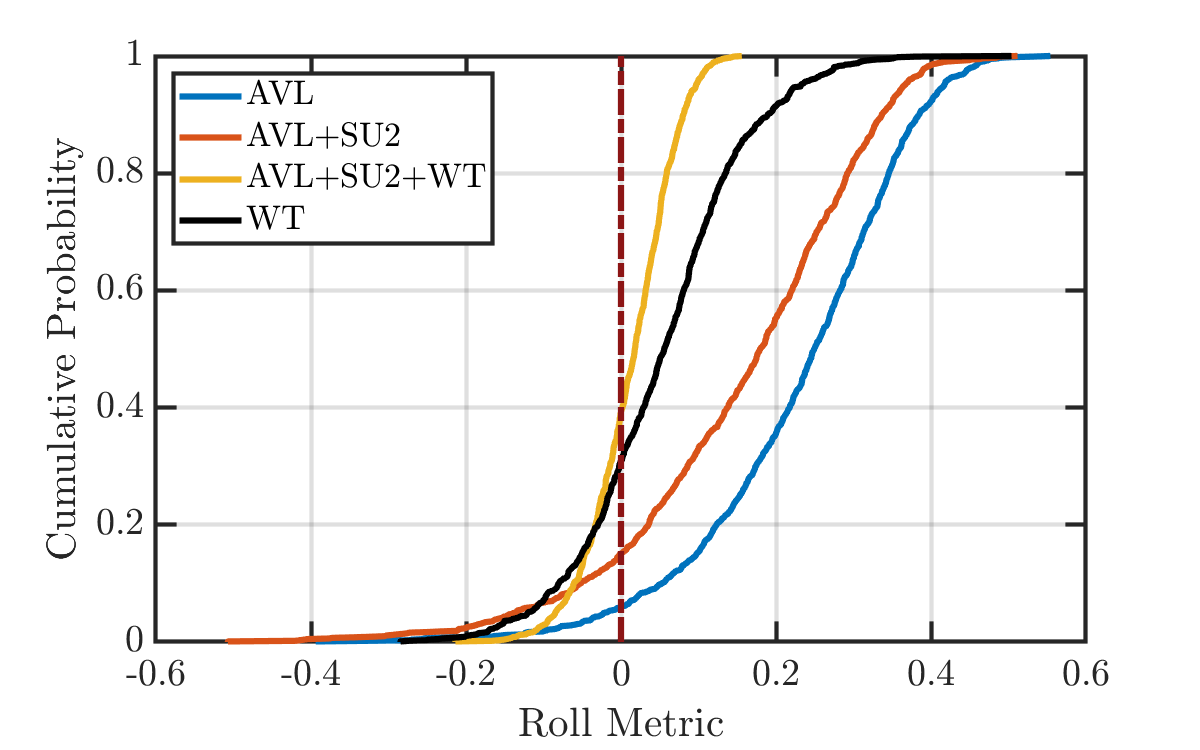
\includegraphics[width=0.75\textwidth]{code/image_gen/cba/Stanford_CFR25_147d_2_R2/images/reo_roll_1f_wt.png}
    \caption{CDF for the roll metric using databases at each fidelity level. \label{fig:reo_roll_all}}
\end{figure}

Current practices would dictate placing an FoS on the deflection limit to account for potential failures due to the uncertainty in the performance predictions.
If the FoS is large, it can result in an overbuilt control surface bigger and bulkier than it needs to be. 
The more critical condition occurs if the FoS is not large enough and the design progresses with insufficient control authority to pass the flight certification tests. 
The later such an issue is recognized, the more expensive a redesign gets. 

The proposed virtual flight testing framework provides success metrics that consider those uncertainties in the design analysis tools. 
Using the CDF output from the simulations and Equations \ref{equ:design_roll_metric}-\ref{equ:design_ail_lim}, engineers can design the control surface to meet a predetermined success rate.
Table \ref{tab:reo_roll_design} lists the current failure rates and the new deflection limits that would be required to achieve a $95\%$ or $100\%$ success rate in the virtual flight testing.

\begin{table}
\centering
    \renewcommand{\arraystretch}{1.2}
    \captionsetup{justification=centering}
    \caption{Certification-based aileron design decisions to achieve prescribed success rate in flight simulations.} 
    \begin{tabular}{|c||c|c|c|}
    \hline
         & Failure Rate & $\delta^{x}_a$ for $x = 95\%$ & $\delta^{x}_a$ for $x = 100\%$ \\ \hline \hline
        AVL & 6.00\% & 15.33 $^\circ$ & 20.91 $^\circ$ \\ \hline 
        AVL+SU2 & 15.10\% & 17.05 $^\circ$ & 22.61 $^\circ$ \\ \hline 
        AVL+SU2+WT & 39.20\% & 16.27 $^\circ$ & 18.21 $^\circ$ \\ \hline 
        WT & 30.80\% & 16.81 $^\circ$ & 19.27 $^\circ$ \\ \hline 
    \end{tabular}
    \label{tab:reo_roll_design}
\end{table}

% A reasonable question to ask would be, why would designers prescribe a success rate lower than $100\%$?

Section \ref{subsec:sf_vs_mf_cba} discussed the general trends seen when adding fidelity levels to the databases.
Those observations are now placed in the context of making certification-based design decisions.
% A few interesting trends can be identified by looking at the different CDF in Figure \ref{fig:reo_roll_all}, and the failure rates and design suggestions in Table \ref{tab:reo_roll_design}.
The low-fidelity databases made using AVL analyses have a low failure rate of $6\%$, but the roll metric covers an extensive range of values.
The AVL analyses over-estimate the effectiveness of the aileron resulting in a lower failure rate. 
However, the significant uncertainties associated with the design analyses propagates through the flight simulation procedure and results in the wide, horizontal spread of the CDF.
Consequently, the $100\%$ design requires a higher deflection limit.

For the AVL+SU2 case, CFD data from SU2 is added to the aerodynamic databases. 
The resulting CDF maintains its shape but shifts towards the three-fidelity (AVL+SU2+WT) and the high-fidelity (WT) case. 
The shift towards a higher failure rate indicates that the baseline aerodynamics databases from AVL were overestimating the aircraft's performance. 
The shape of the CDF remains consistent because the controls databases are identical to the AVL case as there is no CFD-based control derivative information.
These trends are reflected in the higher failure rate and the larger deflection requirements to meet the prescribed success rates. 

Adding high-fidelity wind tunnel data to the aerodynamics and controls databases reduces the uncertainty in the simulation results significantly. 
The relatively small range of values the roll metric achieves, and the steep shape of the CDF for the AVL+SU2+WT case are evidence of this reduction.
The more realistic representation of the flight physics results in a significantly higher failure of $39.2\%$. 
However, the low uncertainty associated with the database results in requiring modest changes to the design to meet the prescribed success rates.
The design requirements are smaller for the three-fidelity case than the high-fidelity case, where the database only relies on only wind tunnel data.
The reason behind the reduction in uncertainty due to the multi-fidelity fit is discussed in Section \ref{subsec:sf_vs_mf_cba} (see Figure \ref{fig:sf_vs_mf_crmail}).

So far, the design variable of choice has been the maximum deflection limit of the control surface. 
However, other design variables, such as aileron size or placement, can also create the same effect.
$\rho_{roll}^x$ acts as a proxy for the supplemental control authority required to achieve the desired success rate. 
The additional control authority can be provided by using larger ailerons or moving the ailerons further outboard on the wing. 
However, in the context of these particular flight simulations, the effect of changing these other design variables is not as straightforward as the effect of changing the deflection limit.
Modifying the simulation to reduce the deflection limits of the aircraft (see Section \ref{subsec:sim_mods}) means that there already existed simulation and experimental data for the effect of the control surface beyond the artificially placed deflection limit. 
If the control surface size or location were changed, it would require rerunning all the design analysis tools to determine the effect of the new aileron design on the aircraft's controls databases. 

Using multi-fidelity modeling and uncertainty quantification to perform virtual flight testing opens new avenues for improving the aircraft design process. 
Flight certification tests can be simulated before building a full-size aircraft prototype, potentially mitigating the enormous costs associated with expensive redesigns late in the aircraft design process.
The probabilistic nature of the simulations also allows for an explicit calculation of failure rates.
This feature can be used to make design decisions to ensure the aircraft can meet the certification requirement with a prescribed success rate. 